\documentclass{article}
\usepackage[utf8]{inputenc}
\usepackage[T1]{fontenc}
\usepackage{authblk}
\usepackage{setspace}
\usepackage{etoolbox}
\usepackage[margin=1in]{geometry}
\usepackage{graphicx}
\graphicspath{ {./figures/} }
\usepackage{subcaption}
\usepackage{amsmath}
\usepackage{amssymb}
\usepackage{url}
\usepackage{float}
\usepackage[font=small,labelfont=bf,labelsep=period]{caption}

% tables and helpers used by the pandoc-converted text
\usepackage{longtable,booktabs,array,calc}
\providecommand{\tightlist}{\setlength{\itemsep}{0pt}\setlength{\parskip}{0pt}}

%%%%%% Bibliography %%%%%%
\usepackage[style=nejm,
citestyle=numeric-comp,
sorting=none,
backend=bibtex]{biblatex}
\addbibresource{references.bib}

\usepackage[hidelinks]{hyperref}

%%%%%% Title %%%%%%
\title{Do AI Models Learn Like Humans?}

%%%%%% Authors %%%%%%
\author[1*]{Somesh Mohapatra}

%%%%%% Affiliations %%%%%%
\affil[1]{Independent.}
\affil[*]{Address correspondence to: pikulsomesh@gmail.com}

\date{}

\setstretch{1.2}
\setlength{\parskip}{0.3em}
\sloppy
\AtBeginEnvironment{longtable}{\small}

\begin{document}

\maketitle

\begin{abstract}
Infants learn a model of their world from a modest amount of experience that arrives once, in order, through senses that start immature and mature on different clocks. Whether these constraints matter for machine learning is usually assumed rather than tested. Here we build a controlled system to test them: one predictive world model per sense (vision, hearing, touch and proprioception) in a synthetic multisensory nursery, each fed through an age-indexed model of sensory immaturity and read out at checkpoints standing for 0, 3, 6 and 12 months, plus a fusion world model that combines them. Six training regimes separate the input schedule, network growth and data order. The input schedule alone reproduces the infant order of sensory maturation, but learning lags well behind what the input allows: at the newborn checkpoint the vision model's toy-position read-out is R\textsuperscript{2} = 0.02, although a supervised network extracts 0.60 from the same input. Growing the network halves training compute and slows learning. Early immaturity improves hearing on clean input (R\textsuperscript{2} 0.45 \ensuremath{\pm} 0.01 versus 0.37 \ensuremath{\pm} 0.04) at a small cost in vision. Fusing the senses tracks a fully hidden toy better than any one sense (R\textsuperscript{2} 0.77 \ensuremath{\pm} 0.06 versus 0.64 \ensuremath{\pm} 0.09 for vision memory). But no model expects a hidden toy to persist: the fused model's apparent surprise disappears when hearing is prevented from giving the event away. In these synthetic models, infant-like input is therefore sufficient for infant-like trajectories of what is decodable, but not for infant-like expectations about hidden objects.
\end{abstract}

\section{Introduction}

By their first birthday, infants expect hidden objects to persist and unsupported objects to fall, attribute goals to agents, and have tuned their perception to the faces and speech sounds around them \autocite{spelke2007core,baillargeon1985object,werker1984cross,pascalis2002species}. They achieve this from a few thousand waking hours of egocentric, repetitive experience that arrives once and in order \autocite{smith2018curriculum}. Self-supervised networks trained on a single child's headcam footage now learn useful visual representations and word meanings \autocite{orhan2020self,orhan2024learning,vong2024grounded}, and expectations about intuitive physics can emerge from video prediction alone \autocite{garrido2025intuitive}. The question this raises is not whether machines can learn from infant data, but whether \textbf{the way infants receive their data} matters for what is learned.

Infant learning differs from standard training in four documented ways. The senses start immature: newborn acuity is about 1 cycle per degree and contrast sensitivity is a small fraction of the adult's \autocite{banks1988optical,norcia1985spatial}. They come online in a fixed order, with touch first, hearing before birth and vision at birth, and this staggered onset may limit competition between the senses \autocite{turkewitz1982limitations}. Plasticity is staggered across senses and levels of the hierarchy \autocite{hensch2005critical,werker2015critical}, and the cortex overproduces synapses and then prunes them rather than adding neurons \autocite{huttenlocher1997regional}. And experience is a single non-stationary stream \autocite{smith2018curriculum}. In networks, initially blurred or achromatic input can make recognition more robust \autocite{vogelsang2018potential,vogelsang2024impact}, slowly changing infant video helps self-supervised learning \autocite{sheybani2023curriculum}, and deep networks show their own critical periods, including for multisensory integration \autocite{achille2019critical,kleinman2023critical}. Yet the benefit of ``starting small'' \autocite{elman1993learning} was challenged by later simulations \autocite{rohde1999language}, curricula help little on standard benchmarks and mainly under limited training budgets or noisy labels \autocite{wu2021curricula}, and stage-like learning can arise from learning dynamics alone \autocite{saxe2019mathematical}.

We therefore treat developmental constraints as hypotheses to test rather than design choices to assume. Nothing in our models is gated by age: no module switches on at a given month, and every capability is measured. We ask four questions, each answered in one section of Results. Do senses mature in the infant order, and is that a property of learning or of the input? Does starting with immature input help? Do combined senses keep information that each sense loses? And do models that can decode a hidden object also expect it to persist?


\section{Materials and Methods}

\hypertarget{experimental-design}{%
\subsection{Experimental design}\label{experimental-design}}

The study compares six training regimes (Table 2) for four sense-specific world models at four checkpoints, with five analyses specified before the final runs: probes at adult-quality, own-age and newborn-quality input; a supervised information ceiling; violation-of-expectation surprise with dissociating events; occluded tracking and fill-in with a fusion model; and planned statistical comparisons (Table 4). Each regime is trained with the same data, the same number of updates and shared hyperparameters.

\hypertarget{environment}{%
\subsection{Environment}\label{environment}}

Episodes last \(T=20\) frames. A toy of type \(c\in\{1,\dots,4\}\) moves with constant velocity and bounces in a 32\ensuremath{\times}32 scene; the hand's position follows a smoothed random motor command \(u_t\in\mathbb R^2\) and stays in the lower half. Half the episodes contain a vertical screen. Vision is an RGB image on a dark background; the toy is drawn with a type-specific shape and colour, the screen in grey and the hand in skin tone. Hearing is a binaural spectrum, \(o^{\text{aud}}_t\in\mathbb R^{2\times32}\), a Gaussian bump at a type-specific pitch whose loudness falls with distance and whose left/right balance follows horizontal position; sound passes through the screen. Touch is an 8\ensuremath{\times}8 image of the toy's shape when the hand overlaps the toy, otherwise zero. Proprioception is the hand's normalised position and velocity. Ground truth includes toy position, type, visibility and contact. Training sets have 3,000 episodes per seed, test sets 400.

\textbf{Probe events.} \emph{Possible}: the toy crosses a central screen horizontally and reappears. \emph{Impossible}: the toy vanishes while hidden, from every sense. \emph{Vanish-visual}: it vanishes from vision and touch but keeps sounding as if still moving. \emph{Silent}: possible and impossible events with no sound at all (hearing receives noise only). \emph{Track}: like possible, with a wider screen (14 px) and varied speed, so the toy is hidden for about seven frames. Paired events share random draws so that they differ only in the manipulation.

\hypertarget{front-ends}{%
\subsection{Front ends}\label{front-ends}}

All front ends are fixed functions \(\tilde o=\Phi_s(o;a)\) whose parameters are linearly interpolated in age from Table 1.

\emph{Vision.} With acuity \(\mathrm{cpd}(a)\) in cycles per degree, contrast sensitivity \(\mathrm{CS}(a)\) and colour saturation \(\gamma(a)\),
\begin{equation}\sigma(a)=\tfrac12\cdot\frac{30}{\mathrm{cpd}(a)}\cdot\frac{32}{224},\qquad x=G_{\sigma(a)}*o,\qquad x\leftarrow \bar x+\kappa(a)\,(x-\bar x),\qquad \kappa(a)=\mathrm{clip}\!\left(\tfrac12\log_{10}\mathrm{CS}(a),\,0.15,\,1\right),\end{equation}
\begin{equation}\tilde o=\mathrm{clip}_{[0,1]}\big(\ell+\gamma(a)(x-\ell)\big),\qquad \ell=0.299x_R+0.587x_G+0.114x_B,\end{equation}
where \(G_\sigma\) is a separable Gaussian with replicate padding and \(\bar x\) the image mean. The log compression of contrast replaces a linear gain \(\mathrm{CS}/100\), which would leave a newborn 2\% of contrast; contrast sensitivity is a threshold, not a gain.

\emph{Hearing.} Per ear, \(x=g_{\beta(a)}*o\) along frequency, then a high-frequency roll-off \(x_f\leftarrow x_f\,\mathrm{sigmoid}\big((h(a)\cdot32-f)/1.5\big)\), then reduced interaural difference \(x_{L,R}\leftarrow m+\rho(a)(x_{L,R}-m)\) with \(m=\tfrac12(x_L+x_R)\), then additive Gaussian noise \(\eta(a)\).

\emph{Touch} and \emph{proprioception.} Receptive-field blur \(G_{\tau(a)}\) on the 8\ensuremath{\times}8 patch plus noise; additive noise on proprioception.

\begin{longtable}[]{@{}
  >{\raggedright\arraybackslash}p{(\columnwidth - 8\tabcolsep) * \real{0.2800}}
  >{\raggedright\arraybackslash}p{(\columnwidth - 8\tabcolsep) * \real{0.1800}}
  >{\raggedright\arraybackslash}p{(\columnwidth - 8\tabcolsep) * \real{0.1800}}
  >{\raggedright\arraybackslash}p{(\columnwidth - 8\tabcolsep) * \real{0.1800}}
  >{\raggedright\arraybackslash}p{(\columnwidth - 8\tabcolsep) * \real{0.2000}}@{}}
\caption{Developmental parameters at the four checkpoints (intermediate months are interpolated).}\tabularnewline
\toprule\noalign{}
\begin{minipage}[b]{\linewidth}\raggedright
Sense
\end{minipage} & \begin{minipage}[b]{\linewidth}\raggedright
0 months
\end{minipage} & \begin{minipage}[b]{\linewidth}\raggedright
3 months
\end{minipage} & \begin{minipage}[b]{\linewidth}\raggedright
6 months
\end{minipage} & \begin{minipage}[b]{\linewidth}\raggedright
12 months
\end{minipage} \\
\midrule\noalign{}
\endfirsthead
\toprule\noalign{}
\begin{minipage}[b]{\linewidth}\raggedright
Sense
\end{minipage} & \begin{minipage}[b]{\linewidth}\raggedright
0 months
\end{minipage} & \begin{minipage}[b]{\linewidth}\raggedright
3 months
\end{minipage} & \begin{minipage}[b]{\linewidth}\raggedright
6 months
\end{minipage} & \begin{minipage}[b]{\linewidth}\raggedright
12 months
\end{minipage} \\
\midrule\noalign{}
\endhead
\bottomrule\noalign{}
\endlastfoot
Vision: acuity (cpd) / contrast sensitivity / colour & 1 / 2 / 0.1 & 4 / 10 / 0.7 & 15 / 50 / 1.0 & 30 / 100 / 1.0 \\
Hearing: frequency blur (bins) / high-frequency pass / interaural difference / noise & 2.5 / 60\% / 0.3 / 0.08 & 1.8 / 75\% / 0.5 / 0.06 & 1.0 / 90\% / 0.8 / 0.04 & 0.5 / 100\% / 1.0 / 0.02 \\
Touch: receptive-field blur (taxels) / noise & 1.2 / 0.06 & 0.9 / 0.04 & 0.6 / 0.03 & 0.3 / 0.02 \\
Proprioception: noise & 0.12 & 0.08 & 0.05 & 0.02 \\
Capacity (growing regimes): width multiplier / memory window & \ensuremath{\times}1 / 1 & \ensuremath{\times}2 / 2 & \ensuremath{\times}3 / 4 & \ensuremath{\times}4 / 6 \\
\end{longtable}

\hypertarget{sense-world-models}{%
\subsection{Sense world models}\label{sense-world-models}}

For sense \(s\) with latent size \(D_s\) (32 for vision, 16 for hearing and touch, 8 for proprioception),
\begin{equation}z_t=e_\theta(\tilde o_t),\qquad \hat z_{t+1}=z_t+f_\theta\big([z_t,z_{t-1},\dots,z_{t-k+1}],u_t\big),\qquad \hat o=d_\theta(z),\end{equation}
where the window is padded with the first frame. The loss on a sub-sequence of 10 frames is
\begin{equation}\mathcal L=\frac{\sum_t w_t\lVert d(z_t)-\tilde o_t\rVert^2}{\sum_t w_t}+\frac{\sum_t w_{t+1}\lVert d(\hat z_{t+1})-\tilde o_{t+1}\rVert^2}{\sum_t w_{t+1}}+0.1\,\lVert\hat z_{t+1}-\mathrm{sg}(z_{t+1})\rVert^2,\end{equation}
with \(\mathrm{sg}\) the stop-gradient. For vision, per-pixel weights \(w=1+20\,\max_c|\tilde o_t-\tilde o_{t-1}|\) up-weight what moves, a stand-in for infants' orienting to motion without which the small toy is ignored. The vision encoder is a three-layer CNN with two coordinate channels and the decoder a spatial-broadcast decoder \autocite{watters2019spatial}; other senses use two-layer MLPs. Widths scale with the multiplier \(w\in\{1,2,3,4\}\).

\textbf{Growth.} \texttt{grow(w\textquotesingle{},\ k\textquotesingle{})} widens every hidden layer as in Box 1 and lengthens the window by adding input weights of zero for the new (older) memory slots, so the model's function is unchanged (verified for every layer by a unit test, \texttt{tests/test\_growth.py}). Vision models grow from 43,507 to 586,499 parameters and hearing models from 13,792 to 149,088.

\textbf{Training.} Adam, learning rate \(2\times10^{-3}\), batch 32, 2,000 updates per stage for vision and 1,500 for other senses, four stages in one continuous run; weights carry over between stages and a fresh Adam optimiser is started at each stage, so all regimes see the same optimiser schedule. Hyperparameters were set once on the immature-input regime and shared by all regimes. Seeds: 3 for each regime (fusion uses the grown regime's checkpoints).

\begin{longtable}[]{@{}
  >{\raggedright\arraybackslash}p{(\columnwidth - 4\tabcolsep) * \real{0.3333}}
  >{\raggedright\arraybackslash}p{(\columnwidth - 4\tabcolsep) * \real{0.3333}}
  >{\raggedright\arraybackslash}p{(\columnwidth - 4\tabcolsep) * \real{0.3333}}@{}}
\caption{Training regimes. All see the same episodes for the same number of updates.}\tabularnewline
\toprule\noalign{}
\begin{minipage}[b]{\linewidth}\raggedright
Regime
\end{minipage} & \begin{minipage}[b]{\linewidth}\raggedright
Network
\end{minipage} & \begin{minipage}[b]{\linewidth}\raggedright
Input quality across the four stages
\end{minipage} \\
\midrule\noalign{}
\endfirsthead
\toprule\noalign{}
\begin{minipage}[b]{\linewidth}\raggedright
Regime
\end{minipage} & \begin{minipage}[b]{\linewidth}\raggedright
Network
\end{minipage} & \begin{minipage}[b]{\linewidth}\raggedright
Input quality across the four stages
\end{minipage} \\
\midrule\noalign{}
\endhead
\bottomrule\noalign{}
\endlastfoot
Immature input (primary) & fixed (12-month size) & 0 \ensuremath{\rightarrow} 3 \ensuremath{\rightarrow} 6 \ensuremath{\rightarrow} 12 months \\
Immature input + growth & grows \ensuremath{\times}1 \ensuremath{\rightarrow} \ensuremath{\times}4 & 0 \ensuremath{\rightarrow} 3 \ensuremath{\rightarrow} 6 \ensuremath{\rightarrow} 12 \\
Growth only & grows \ensuremath{\times}1 \ensuremath{\rightarrow} \ensuremath{\times}4 & adult throughout \\
Adult input & fixed & adult throughout \\
Shuffled input quality & fixed & each batch from a random stage \\
Reversed immaturity & fixed & 12 \ensuremath{\rightarrow} 6 \ensuremath{\rightarrow} 3 \ensuremath{\rightarrow} 0 \\
\end{longtable}

\hypertarget{fusion-world-model}{%
\subsection{Fusion world model}\label{fusion-world-model}}

Given frozen sense latents \(z^s_t\) and a mask \(m^s_t\in\{0,1\}\),
\begin{equation}h_t=\mathrm{MLP}\!\left(\frac{\sum_s m^s_t\,(P_s z^s_t+\epsilon_s)}{\max(1,\sum_s m^s_t)}\right),\qquad \hat h_{t+1}=h_t+g\big([h_t,\dots,h_{t-5}],u_t\big),\end{equation}
with projections \(P_s\) to 64 dimensions and learned modality embeddings \(\epsilon_s\). Read-out heads \(r_s\) reconstruct every sense latent from \(h_t\) and from \(\hat h_{t+1}\):
\begin{equation}\mathcal L_{\text{fus}}=\frac1{|S|}\sum_s\Big(\lVert r_s(h_t)-z^s_t\rVert^2+\lVert r_s(\hat h_{t+1})-z^s_{t+1}\rVert^2\Big),\end{equation}
with each sense dropped independently with probability 0.3 during training. Latents are standardised per sense.

\hypertarget{read-outs}{%
\subsection{Read-outs}\label{read-outs}}

\textbf{Linear probes.} For features \(X\) (a latent, or a memory window of latents) and targets \(Y\), ridge regression with centred targets and an unpenalised intercept,
\begin{equation}\hat B=\arg\min_B\lVert (Y-\bar Y)-X_cB\rVert^2+\lambda\lVert B\rVert^2=(X_c^\top X_c+\lambda I)^{-1}X_c^\top(Y-\bar Y),\end{equation}
with \(X_c\) standardised features, is fitted on training episodes and evaluated on test episodes, \(R^2=1-\sum\lVert y-\hat y\rVert^2/\sum\lVert y-\bar y\rVert^2\). Identity uses one-hot targets and the arg-max (chance 0.25). Touch is probed on contact frames, proprioception on hand position. \emph{Adult-input} probes use adult-quality input; \emph{own-age} probes use the input quality of the checkpoint's age; \emph{newborn-input} probes are fitted on adult-quality input and tested on newborn-quality input.

\textbf{Information ceiling.} For each sense and age \(a\in\{0,1,2,3,4,6,9,12\}\), a supervised network (the same encoder family) is trained for 1,500 updates to predict toy position and identity from a single filtered frame, and evaluated on held-out frames.

\textbf{Violation of expectation.} Surprise is one-step prediction error, \(S_t=\lVert d(\hat z_t)-\tilde o_t\rVert^2\) (unimodal) or \(\lVert r_s(\hat h_t)-z^s_t\rVert^2\) per channel (fused, standardised latents), averaged over the hidden stretch and the two frames after expected re-emergence. With \(S_{\text{pos}}\) and \(S_{\text{imp}}\) the mean surprise on paired possible and impossible events,
\begin{equation}\mathrm{VoE}=\frac{S_{\text{imp}}-S_{\text{pos}}}{S_{\text{imp}}+S_{\text{pos}}},\qquad d_z=\frac{\overline{S_{\text{imp}}-S_{\text{pos}}}}{\mathrm{sd}(S_{\text{imp}}-S_{\text{pos}})}.\end{equation}

\textbf{Occluded tracking and fill-in.} The hidden toy's horizontal position is probed on fully hidden frames of the \emph{track} events from the vision model's memory window (\(k=6\) latents), from the hearing latent, and from the fused state, fitting on half of the episodes and testing on the other half. Fill-in probes toy position from the fused state with all senses, without vision, and from single senses.

\textbf{Statistics.} Bands and whiskers are \ensuremath{\pm}1 s.d. over seeds. Planned comparisons at the 12-month checkpoint use Welch's t-test and Hedges' \(g=\frac{\bar a-\bar b}{s_p}\big(1-\frac{3}{4(n_a+n_b)-9}\big)\) with approximate 95\% interval \(g\pm1.96\sqrt{\frac{n_a+n_b}{n_an_b}+\frac{g^2}{2(n_a+n_b)}}\); per-cell 95\% bootstrap intervals are in \texttt{results/extra.json}. No correction for multiple comparisons is applied; we list all planned comparisons.

\begin{longtable}[]{@{}llll@{}}
\caption{Planned comparisons.}\tabularnewline
\toprule\noalign{}
Comparison (12-month checkpoint) & Hedges' g & p (Welch) & n \\
\midrule\noalign{}
\endfirsthead
\toprule\noalign{}
Comparison (12-month checkpoint) & Hedges' g & p (Welch) & n \\
\midrule\noalign{}
\endhead
\bottomrule\noalign{}
\endlastfoot
Vision clean, immature vs adult input & \ensuremath{-}1.0 & 0.21 & 3/3 \\
Vision clean, grown vs immature & \ensuremath{-}0.8 & 0.32 & 3/3 \\
Vision identity, grown vs immature & \ensuremath{-}2.2 & 0.05 & 3/3 \\
Vision on newborn input, immature vs adult & 0.6 & 0.46 & 3/3 \\
Hearing clean, immature vs adult & 2.3 & 0.06 & 3/3 \\
Hearing clean, grown vs growth only & 1.9 & 0.10 & 3/3 \\
Hidden toy, fused vs vision memory & 1.4 & 0.11 & 3/3 \\
\end{longtable}

\textbf{Compute.} Training compute is approximated by \(\sum_{\text{stages}}(\text{parameters})\times(\text{updates})\); relative to a fixed 12-month-size network, grown vision models use 0.48 and grown hearing models 0.49.

\textbf{Milestones.} For each sense, the half-ceiling age is the first age at which the ceiling reaches half of its 12-month value (position R\textsuperscript{2} for vision and hearing; identity accuracy above chance for touch). Kendall's \ensuremath{\tau} compares the resulting order with the order of functional maturity usually described for the three senses, touch before hearing before vision \autocite{turkewitz1982limitations}.

\textbf{Human and animal studies.} The study uses only synthetic data; no human or animal participants were involved.

\textbf{Code and data availability.} All code, configurations, results and trained checkpoints are at \url{https://github.com/pikulsomesh/developmental-world-models} (MIT licence). \texttt{scripts/run\_experiments.py} trains every regime, \texttt{scripts/analyze\_fusion\_voe.py} and \texttt{scripts/analyze\_extra.py} run the analyses, \texttt{scripts/make\_paper\_figures.py} draws the figures, and \texttt{scripts/fill\_report.py} writes every number in this report from the results files. An interactive companion and wiki are at \url{https://pikulsomesh.github.io/developmental-world-models/}. Code and results of the companion studies are in \texttt{companion/age-modeling} and \texttt{companion/cross-sense}.


\section{Results}

\hypertarget{a-testbed-of-sense-specific-developmental-world-models}{%
\subsection{A testbed of sense-specific developmental world models}\label{a-testbed-of-sense-specific-developmental-world-models}}

\begin{figure}[tbp]
\centering
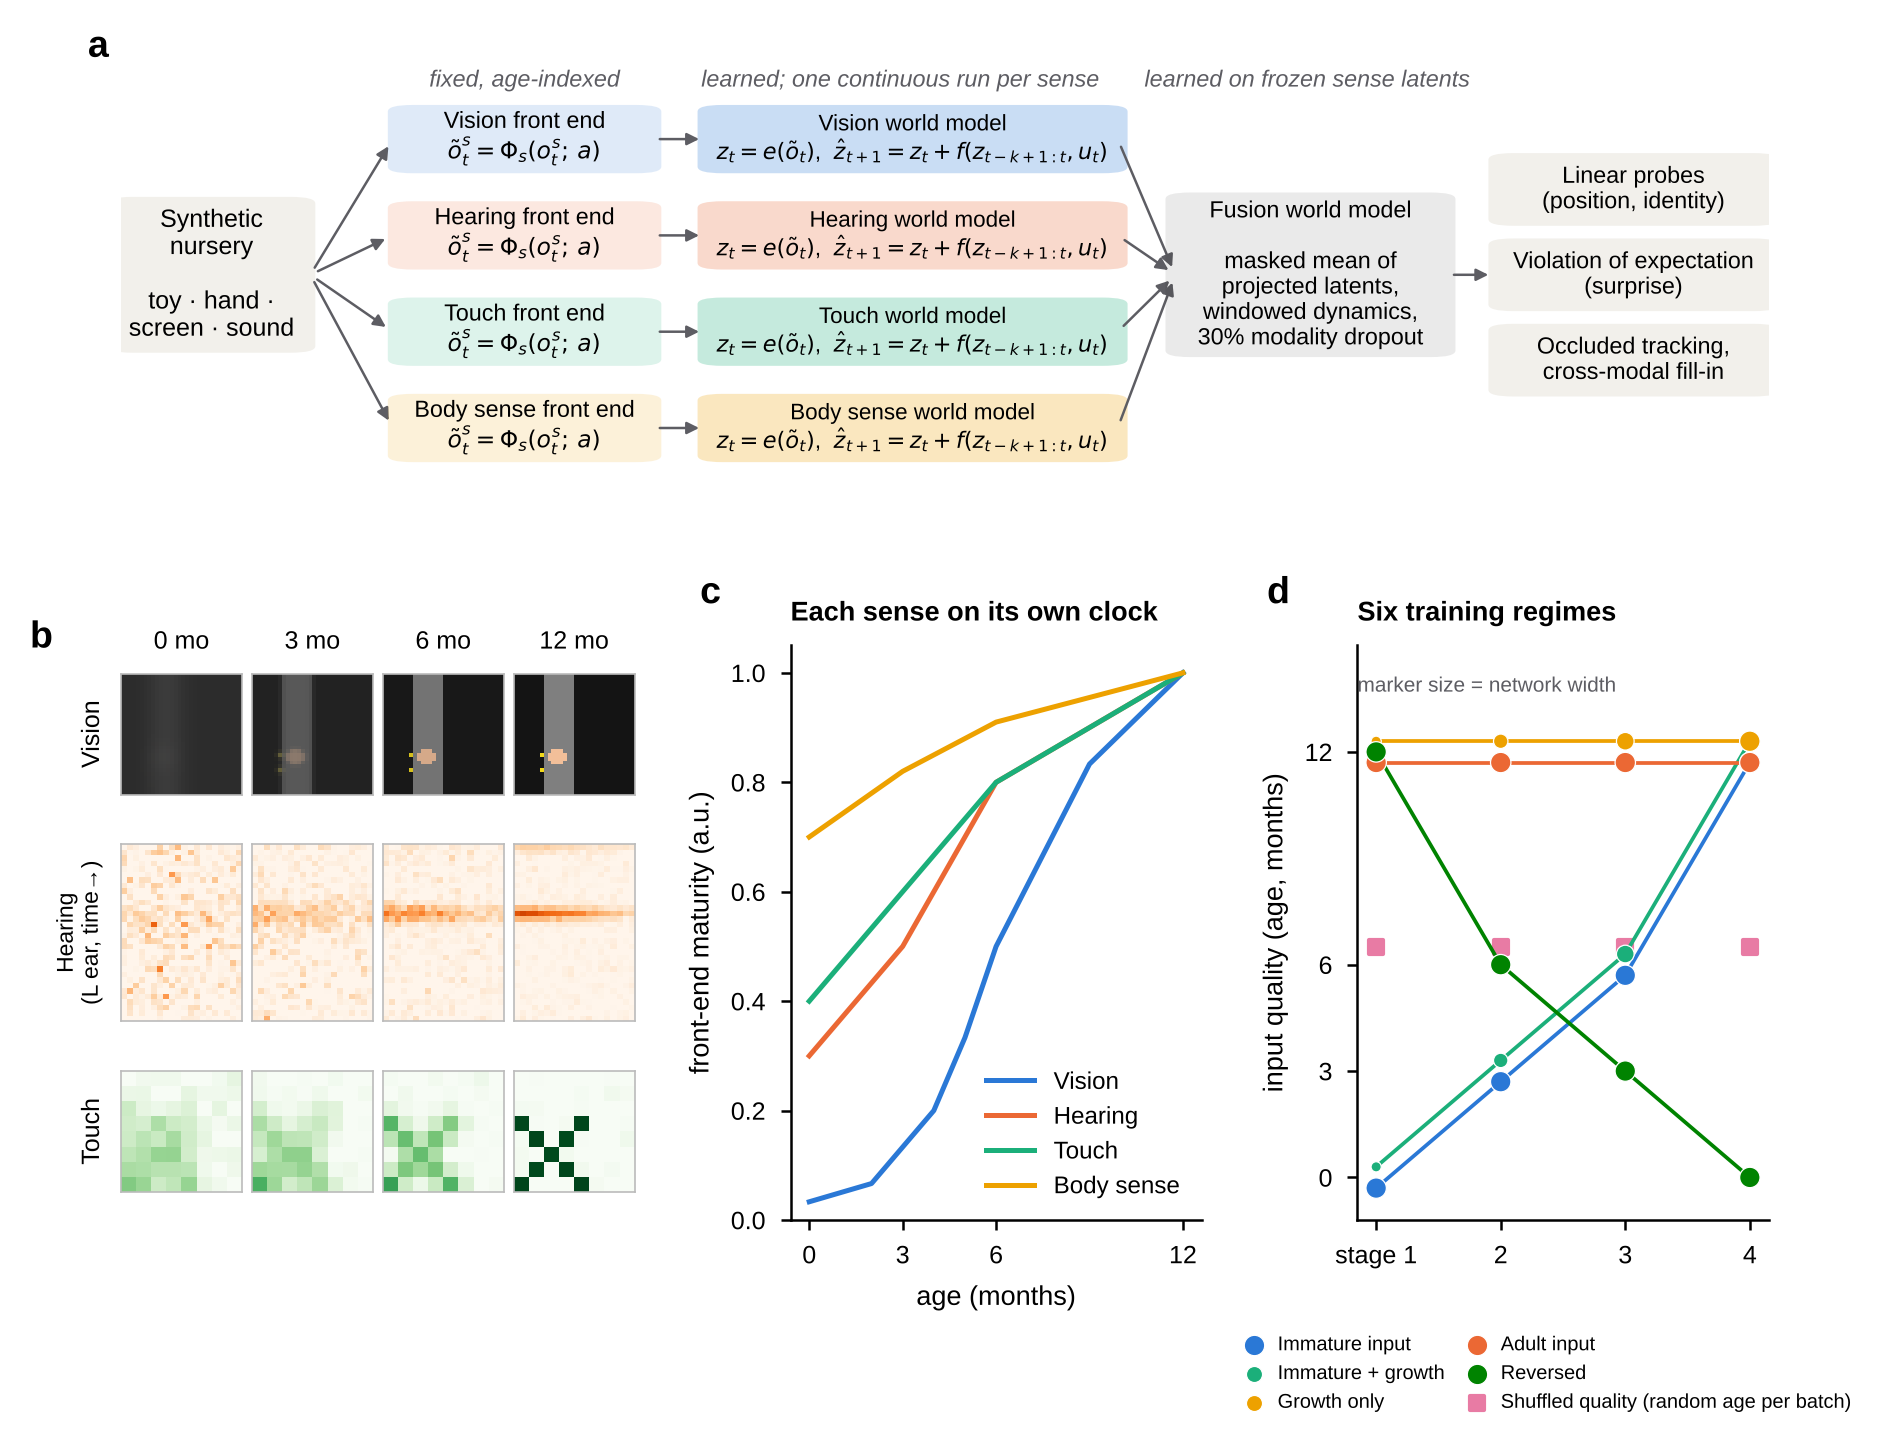
\includegraphics[width=\textwidth,height=0.78\textheight,keepaspectratio]{fig1_overview.png}
\caption{\textbf{Sense-specific developmental world models.} \textbf{a}, Each sense passes a synthetic nursery (a toy that is seen, heard and felt, the infant's babbling hand, and an occluding screen) through a fixed, age-indexed front end \(\Phi_s(\cdot;a)\), and learns its own world model: an encoder \(e\), a dynamics model \(f\) over the last \(k\) latents and the infant's motor command \(u_t\), and a decoder. A fusion world model combines the frozen sense latents. Read-outs are linear probes, violation-of-expectation surprise and occluded tracking. \textbf{b}, The same moment delivered to vision, hearing (left ear, 32 frequency bins over the episode) and touch (an 8\ensuremath{\times}8 patch of skin) at 0, 3, 6 and 12 months. \textbf{c}, Front-end maturity per sense (normalised parameters of Table 1): touch and proprioception start close to mature, hearing partly, vision far behind. \textbf{d}, The six training regimes: input quality over the four training stages; marker size is network width.}
\end{figure}

The nursery (Fig. 1a; Methods) renders one toy of four types, a babbling hand and, in half the scenes, a vertical screen into four streams: 32\ensuremath{\times}32 colour vision, binaural hearing (2 ears \ensuremath{\times} 32 frequency bins, panned by position and passing through the screen), an 8\ensuremath{\times}8 tactile patch on the hand, and four-dimensional proprioception. Each toy type is specified redundantly across senses, by shape and colour, pitch, and felt shape \autocite{bahrick2000intersensory}.

Each sense is filtered by a fixed front end whose parameters follow the age \(a\) (Fig. 1b, c; Table 1). For vision we use published infant acuity and contrast sensitivity \autocite{norcia1985spatial,banks1988optical}; for hearing, touch and proprioception we use coarse placeholder tables that respect the known order of maturation. Behind each front end is a world model of the same family (Methods): an encoder, a residual dynamics model over a memory window, and a decoder, trained to reconstruct the current observation and predict the next one. Each sense is trained in one continuous run of four stages and read out at the end of each stage; we call these checkpoints 0, 3, 6 and 12 months. Six regimes (Fig. 1d; Table 2) cross two levers, the input schedule and network growth, with two order controls. All regimes see the same data for the same number of updates.

\hypertarget{the-input-schedule-sets-the-order-learning-lags-the-input}{%
\subsection{The input schedule sets the order; learning lags the input}\label{the-input-schedule-sets-the-order-learning-lags-the-input}}

\begin{figure}[tbp]
\centering
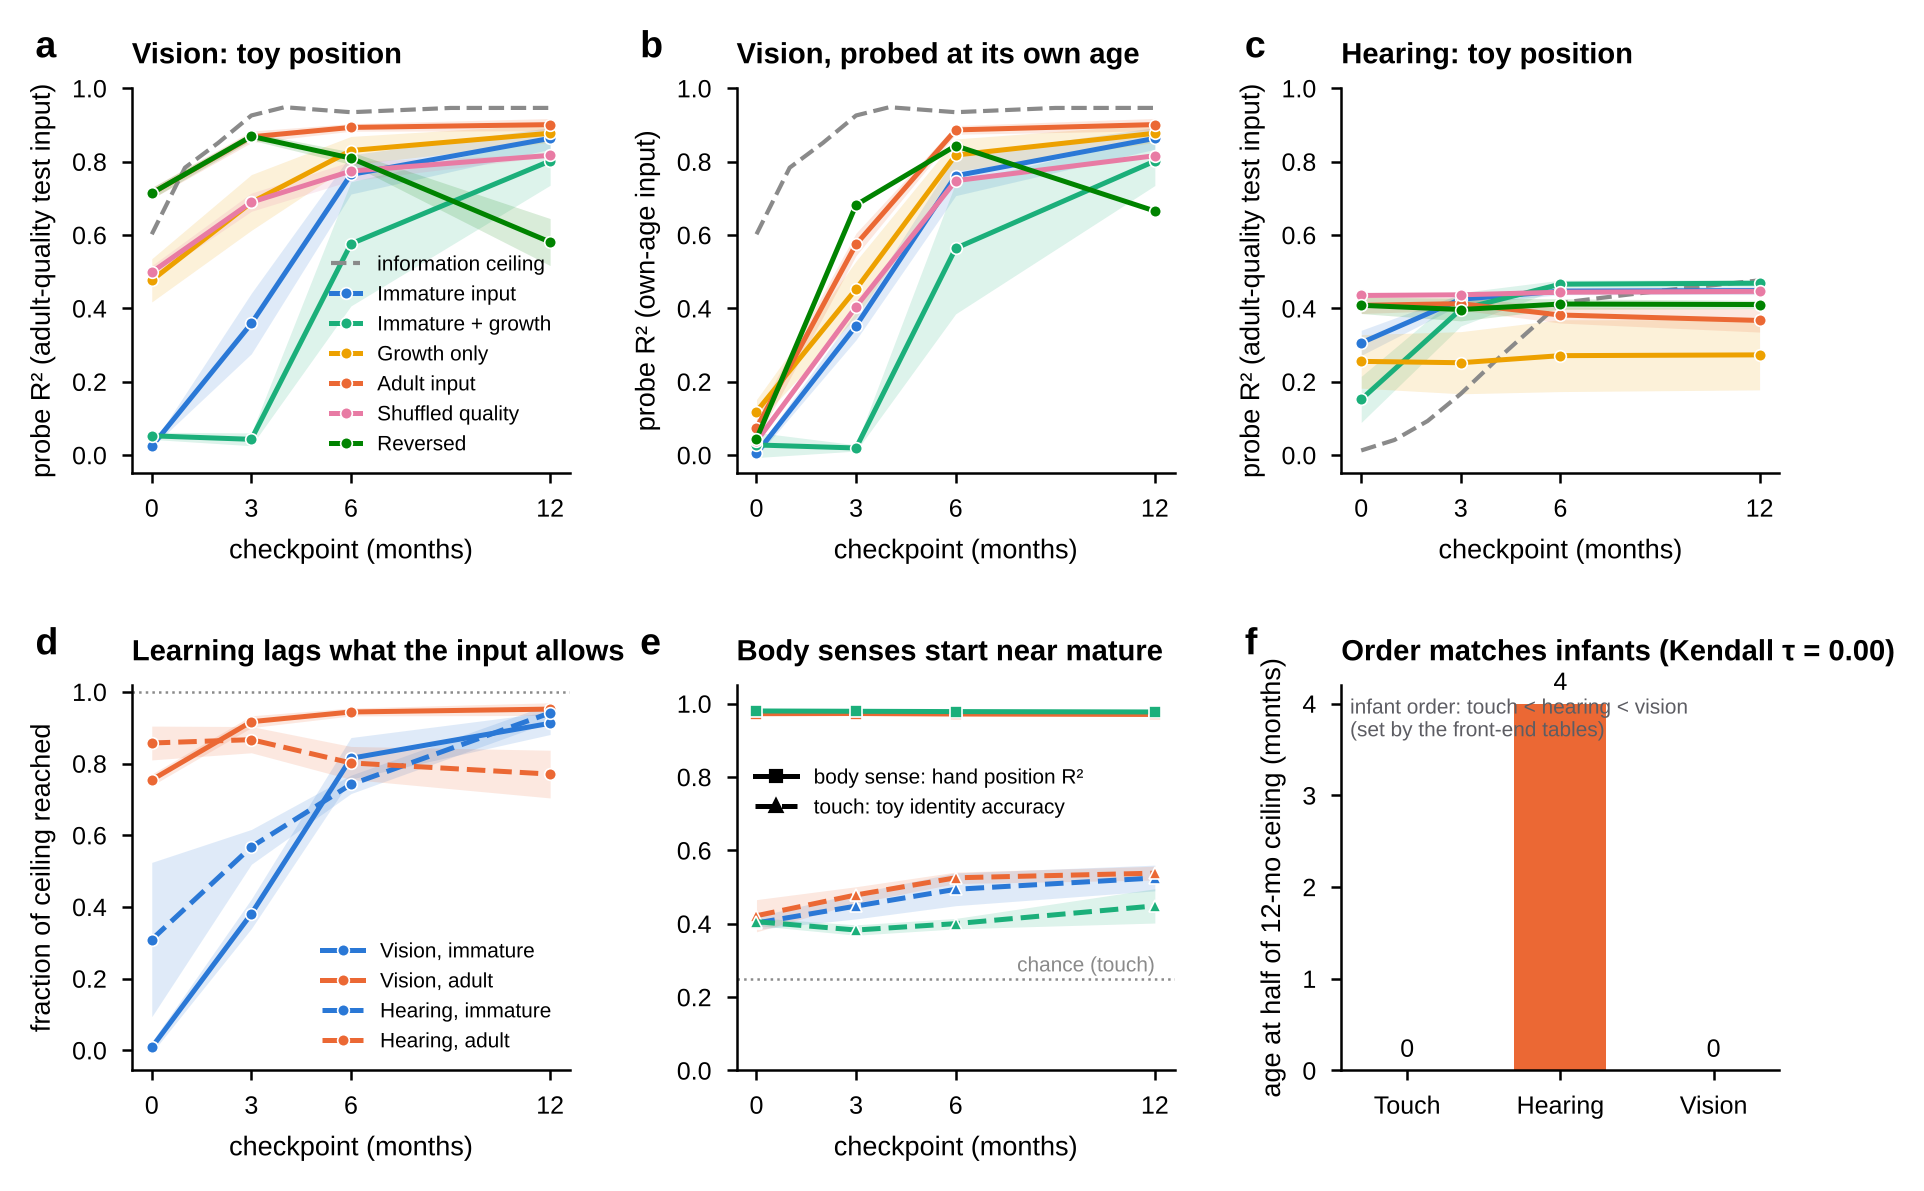
\includegraphics[width=\textwidth,height=0.78\textheight,keepaspectratio]{fig2_development.png}
\caption{\textbf{Development of each sense.} \textbf{a}, Toy position decoded from the vision model's latent at each checkpoint (probe fitted and tested on adult-quality input), for the six regimes; dashed grey line, information ceiling (a supervised network trained directly on that age's filtered input). \textbf{b}, The same with the probe fitted and tested on the input quality of the checkpoint's own age. \textbf{c}, Hearing. \textbf{d}, Fraction of the age-matched ceiling reached by the immature-input regime (own-age probe) and by the adult-input regime, for vision (solid) and hearing (dashed). \textbf{e}, Proprioception (hand position R\textsuperscript{2}, squares) and touch (toy identity accuracy, triangles; chance 0.25) are close to their final level from the first checkpoint. \textbf{f}, Age at which each sense's ceiling first reaches half its 12-month value; the order matches infants, by construction of the front-end tables. Lines, mean over seeds; bands, \ensuremath{\pm}1 s.d.; n = 3 seeds per regime.}
\end{figure}

With immature input, the vision model cannot localise the toy at the first two checkpoints (position R\textsuperscript{2} 0.02 \ensuremath{\pm} 0.00 and 0.36 \ensuremath{\pm} 0.10) and then rises steeply to 0.86 \ensuremath{\pm} 0.04 (Fig. 2a). The same network trained on adult-quality input localises the toy from the first checkpoint (0.71 \ensuremath{\pm} 0.02) and ends at 0.90 \ensuremath{\pm} 0.02. Hearing rises modestly as binaural cues mature, and proprioception and touch are near their final level throughout (Fig. 2c, e). The infant order of maturation, body senses first, hearing next, vision last, therefore appears; half-ceiling ages are touch 0, hearing 4 and vision 0 months (Kendall \ensuremath{\tau} = 0.00 against the infant order; Fig. 2f). This agreement is put there by the front-end tables and is not a finding about learning.

Two controls separate learning from input. First, probing on adult-quality input asks a model trained on blurred images to generalise to sharp ones. Probing instead on each checkpoint's own input (Fig. 2b) gives 0.00 \ensuremath{\pm} 0.01 at 0 months and 0.86 \ensuremath{\pm} 0.04 at 12, so the early failure is not a distribution-shift artefact. Second, the newborn input is not empty: a supervised network trained directly on it decodes toy position with R\textsuperscript{2} = 0.60, rising to 0.95 at 12 months (Fig. 2a, dashed). The self-supervised vision model reaches only a small fraction of what its input allows at the early checkpoints and closes the gap later (Fig. 2d). The infant-like curve is thus a joint product of what the input contains and how slowly a predictive objective extracts a small object from a blurred, low-contrast scene.

\hypertarget{growth-slows-learning-and-halves-compute}{%
\subsection{Growth slows learning and halves compute}\label{growth-slows-learning-and-halves-compute}}

Adding growth to immature input does not change the shape of the curve; it delays it (Fig. 2a). The grown vision model is still at R\textsuperscript{2} 0.04 \ensuremath{\pm} 0.02 at the 3-month checkpoint and ends at 0.80 \ensuremath{\pm} 0.08, against 0.86 \ensuremath{\pm} 0.04 for the fixed-size network; identity accuracy is 0.50 \ensuremath{\pm} 0.08 against 0.67 \ensuremath{\pm} 0.04 (Hedges' g = \ensuremath{-}2.2, p = 0.05). Growth without immature input learns quickly and ends near the adult-input model (0.88 \ensuremath{\pm} 0.03). At matched updates, growing networks use 0.48 of the fixed network's parameter-updates (Fig. 3d). The delay has a simple cause (Box 1): units added with zero outgoing weights receive zero gradient on their incoming weights until the outgoing weights move, so new capacity contributes nothing at first.

\hypertarget{early-immaturity-a-small-cost-in-vision-a-benefit-in-hearing}{%
\subsection{Early immaturity: a small cost in vision, a benefit in hearing}\label{early-immaturity-a-small-cost-in-vision-a-benefit-in-hearing}}

\begin{figure}[tbp]
\centering
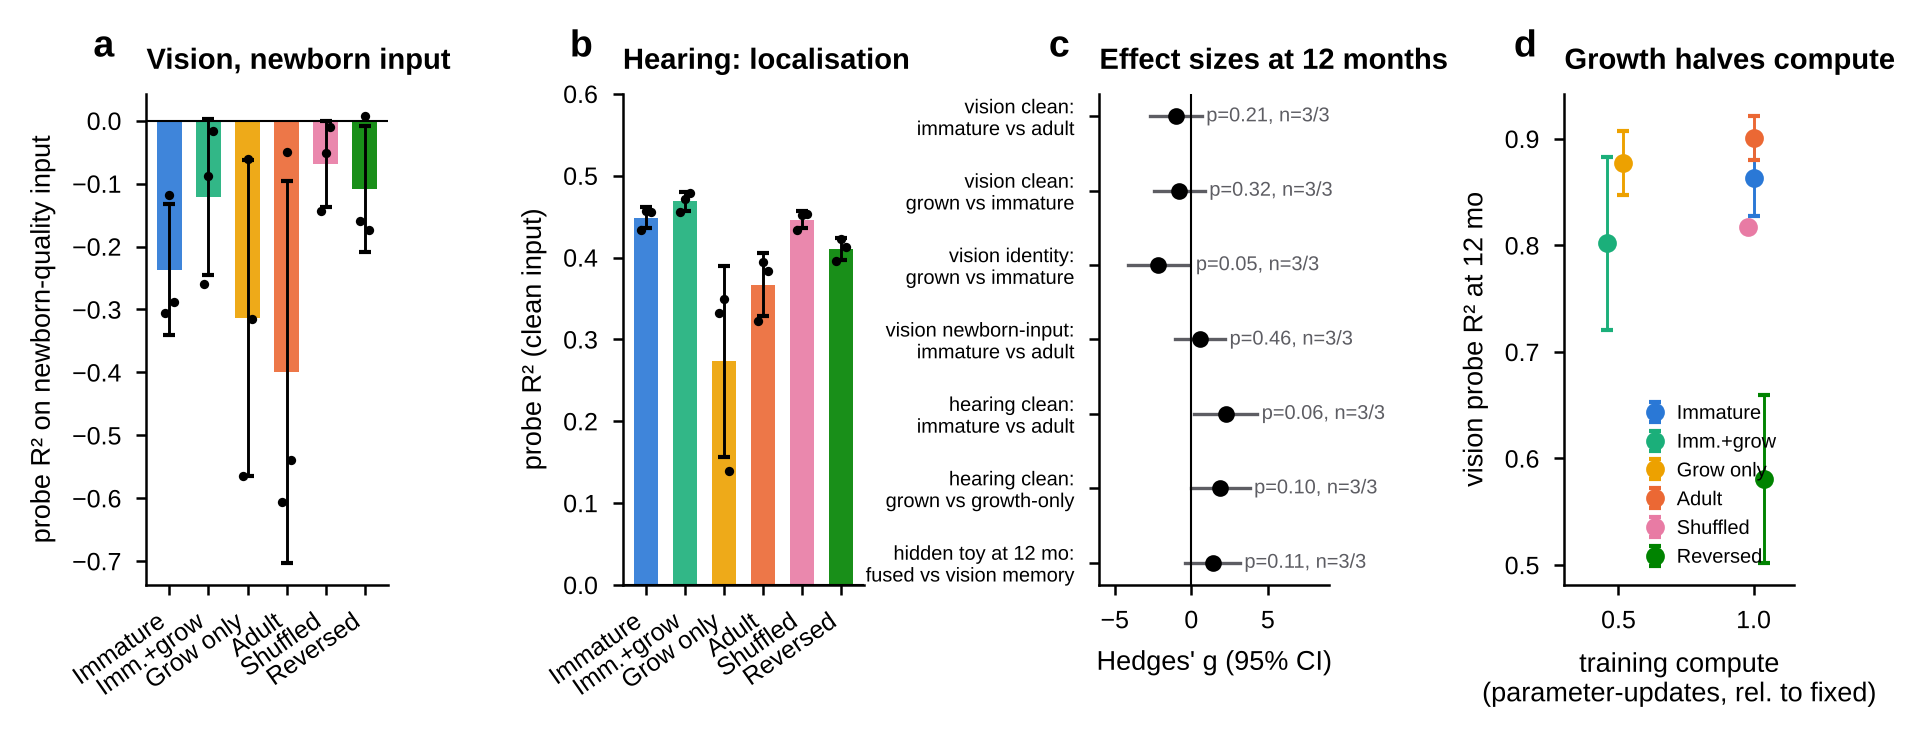
\includegraphics[width=\textwidth,height=0.78\textheight,keepaspectratio]{fig3_costs_benefits.png}
\caption{\textbf{Costs and benefits at the 12-month checkpoint.} \textbf{a}, Vision probe R\textsuperscript{2} when tested on newborn-quality input (bars, mean; dots, seeds; whiskers, s.d.). All values are negative (worse than predicting the mean), so differences are in how badly models fail. \textbf{b}, Hearing localisation on clean input. \textbf{c}, Effect sizes (Hedges' g with approximate 95\% CI) and Welch-test p values for the planned comparisons; n per group shown. \textbf{d}, Vision accuracy against training compute (parameter-updates relative to a fixed-size network).}
\end{figure}

On clean input the adult-input vision model is best. Immature input costs 0.90 \ensuremath{-} 0.86 in R\textsuperscript{2} (g = \ensuremath{-}1.0, p = 0.21). Tested on newborn-quality input, every model fails (Fig. 3a), with regimes that saw immature input failing less on average (\ensuremath{-}0.24 \ensuremath{\pm} 0.10 against \ensuremath{-}0.40 \ensuremath{\pm} 0.30 for adult input), but the difference is within seed variability (p = 0.46). We do not claim a robustness benefit in vision.

Hearing is different. Models that heard immature sound early localise better on clean input at 12 months (0.45 \ensuremath{\pm} 0.01 immature, 0.47 \ensuremath{\pm} 0.01 immature with growth) than models that only heard adult-quality sound (0.37 \ensuremath{\pm} 0.04 adult input, 0.27 \ensuremath{\pm} 0.12 growth only; Fig. 3b; g = 2.3, p = 0.06). Shuffled input quality (0.45 \ensuremath{\pm} 0.01) is close to the immature schedule, which suggests that the benefit comes from having heard degraded input at all, a form of augmentation, more than from its order. Reversing the schedule is the clearest negative control: the vision model that ends on newborn-quality input falls from 0.87 \ensuremath{\pm} 0.01 to 0.58 \ensuremath{\pm} 0.08.

\hypertarget{combined-senses-keep-what-each-sense-loses}{%
\subsection{Combined senses keep what each sense loses}\label{combined-senses-keep-what-each-sense-loses}}

\begin{figure}[tbp]
\centering
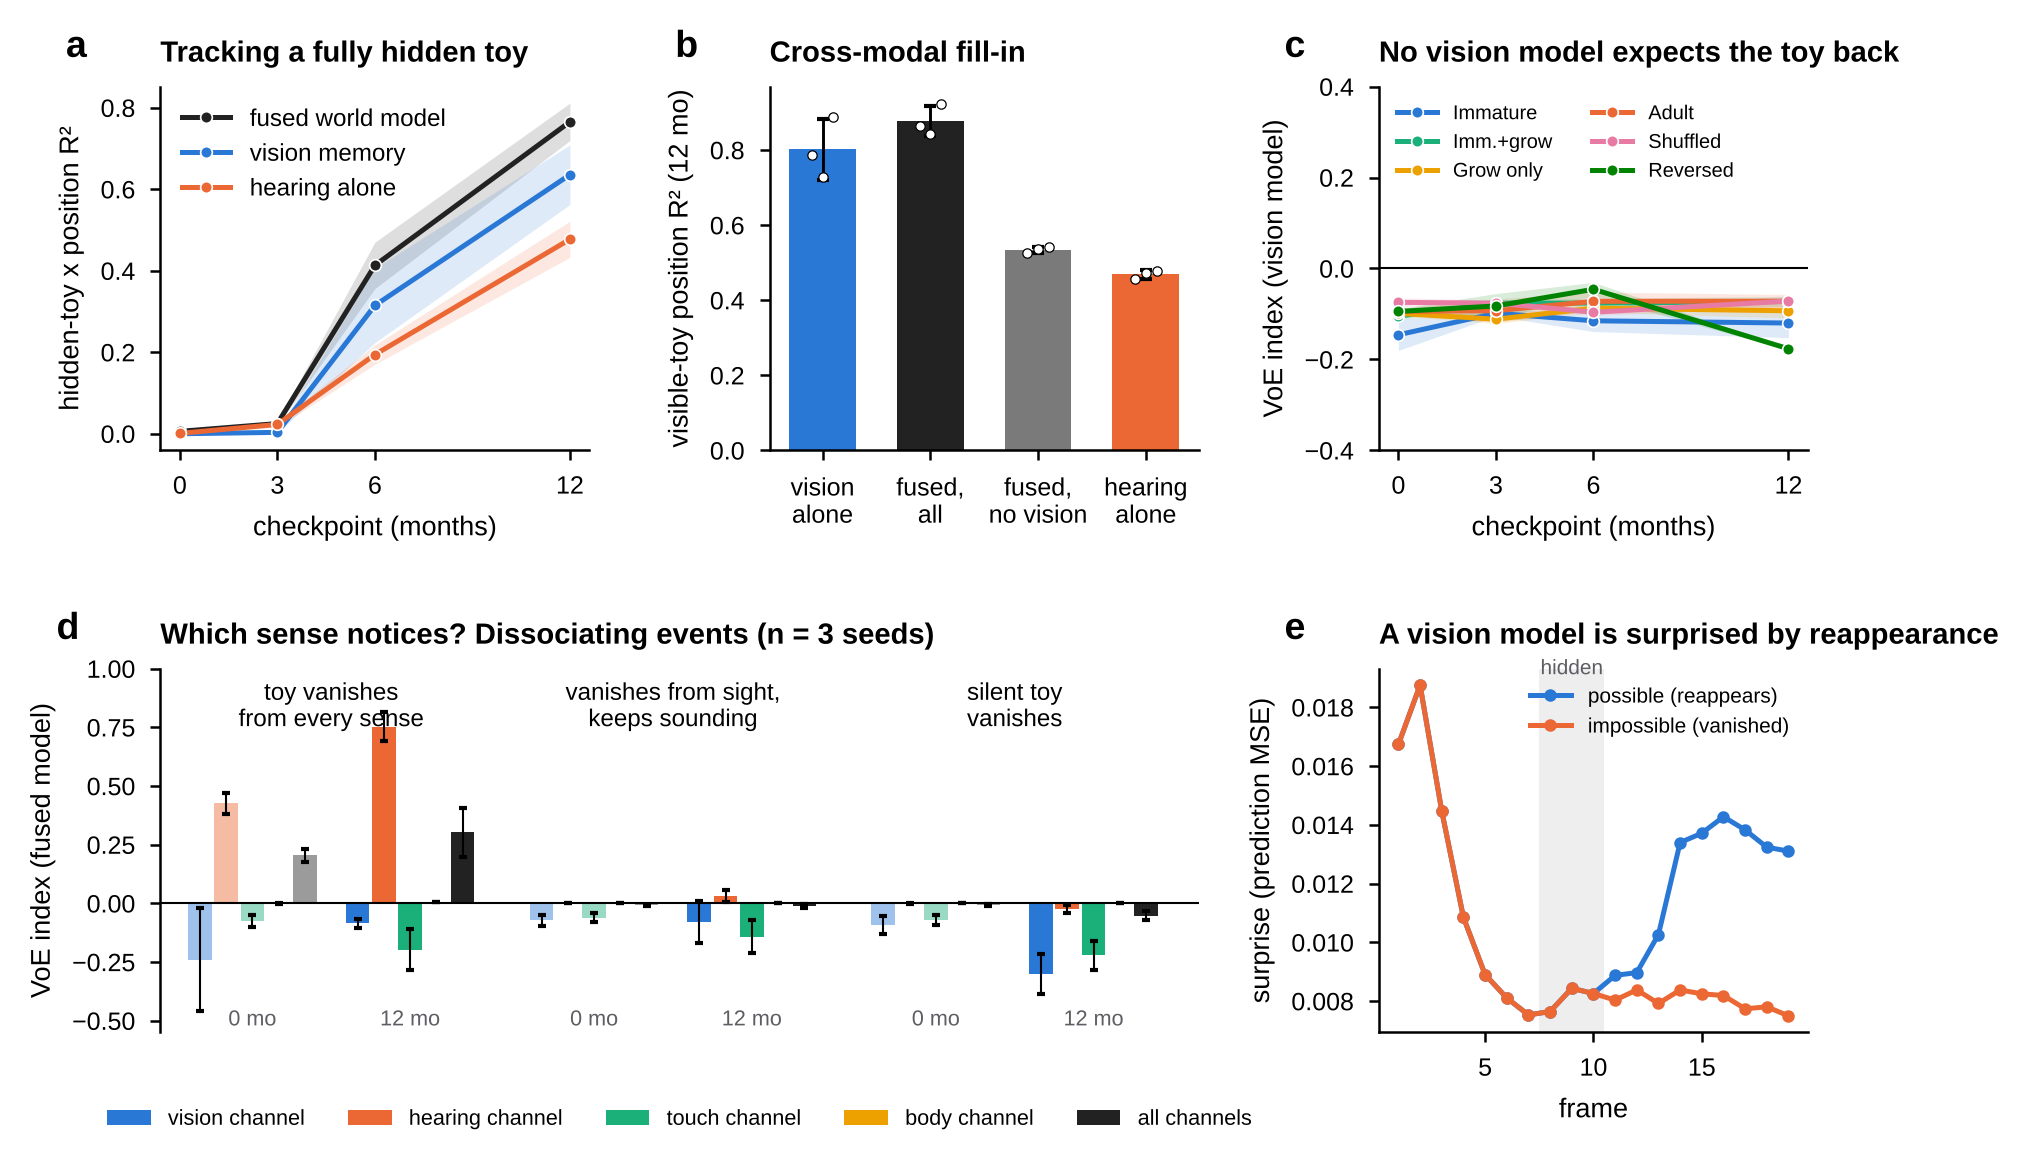
\includegraphics[width=\textwidth,height=0.78\textheight,keepaspectratio]{fig4_fusion_expectation.png}
\caption{\textbf{Fusion and expectation.} \textbf{a}, Horizontal position of a fully hidden toy decoded from the vision model's memory window, from hearing alone and from the fused world model. \textbf{b}, Position of a visible toy at 12 months from vision alone, the fused state, the fused state with vision switched off, and hearing alone. \textbf{c}, Violation-of-expectation (VoE) index of the unimodal vision models; positive means more surprise when the toy fails to reappear. \textbf{d}, VoE index of the fused model broken down by channel, for three events: the toy vanishes from every sense; it vanishes from sight and touch but keeps sounding; a silent toy vanishes. Faded bars, 0 months; solid, 12 months. \textbf{e}, Frame-by-frame surprise of one vision model (immature input, 12 months) on a possible and an impossible event; grey, toy hidden. Bands and whiskers, \ensuremath{\pm}1 s.d. over seeds.}
\end{figure}

During a long occlusion, the hidden toy's horizontal position can be decoded from the vision model's memory (R\textsuperscript{2} 0.64 \ensuremath{\pm} 0.09 at 12 months), from hearing, which passes through the screen (0.48 \ensuremath{\pm} 0.05), and best from the fused world model (0.77 \ensuremath{\pm} 0.06; Fig. 4a; paired difference fused minus vision positive in every seed). The advantage appears at 6 months and nothing is decodable at 0 to 3 months, when neither vision nor binaural hearing can localise. For a visible toy, the fused state is better than vision alone (0.88 \ensuremath{\pm} 0.04 against 0.80 \ensuremath{\pm} 0.08) and, with vision switched off, still recovers position from hearing, touch and the hand (0.53 \ensuremath{\pm} 0.01; Fig. 4b).

\hypertarget{decodable-is-not-expected}{%
\subsection{Decodable is not expected}\label{decodable-is-not-expected}}

No unimodal vision model, in any regime, has a positive VoE index (Fig. 4c): all are more surprised when the toy reappears than when it fails to, like a predictor that copies the last frame (Fig. 4e). This holds although the hidden toy's position is decodable from the same model's memory. Squared-error prediction explains it (Box 1): the error-minimising forecast is the conditional mean of the next frame, and when the reappearance time is uncertain that mean is dominated by the screen.

The fused model does show a positive index when the toy vanishes from every sense (0.30 \ensuremath{\pm} 0.10 at 12 months), but its channels show where the surprise comes from: hearing 0.75 \ensuremath{\pm} 0.06, vision \ensuremath{-}0.09 \ensuremath{\pm} 0.02 (Fig. 4d). The model notices that the sound stopped. When the toy vanishes from sight but keeps sounding, the overall index is \ensuremath{-}0.01 \ensuremath{\pm} 0.01 and the vision channel \ensuremath{-}0.08 \ensuremath{\pm} 0.09; when a silent toy vanishes, they are \ensuremath{-}0.05 \ensuremath{\pm} 0.02 and \ensuremath{-}0.30 \ensuremath{\pm} 0.09. Without a sound to give the event away, the fused model does not expect the toy back either. A read-out can show that information about a hidden object is present while the model's predictions do not use it; object permanence has to be tested with paradigms, not probes.

\hypertarget{convergent-evidence-from-two-companion-studies}{%
\subsection{Convergent evidence from two companion studies}\label{convergent-evidence-from-two-companion-studies}}

\begin{figure}[tbp]
\centering
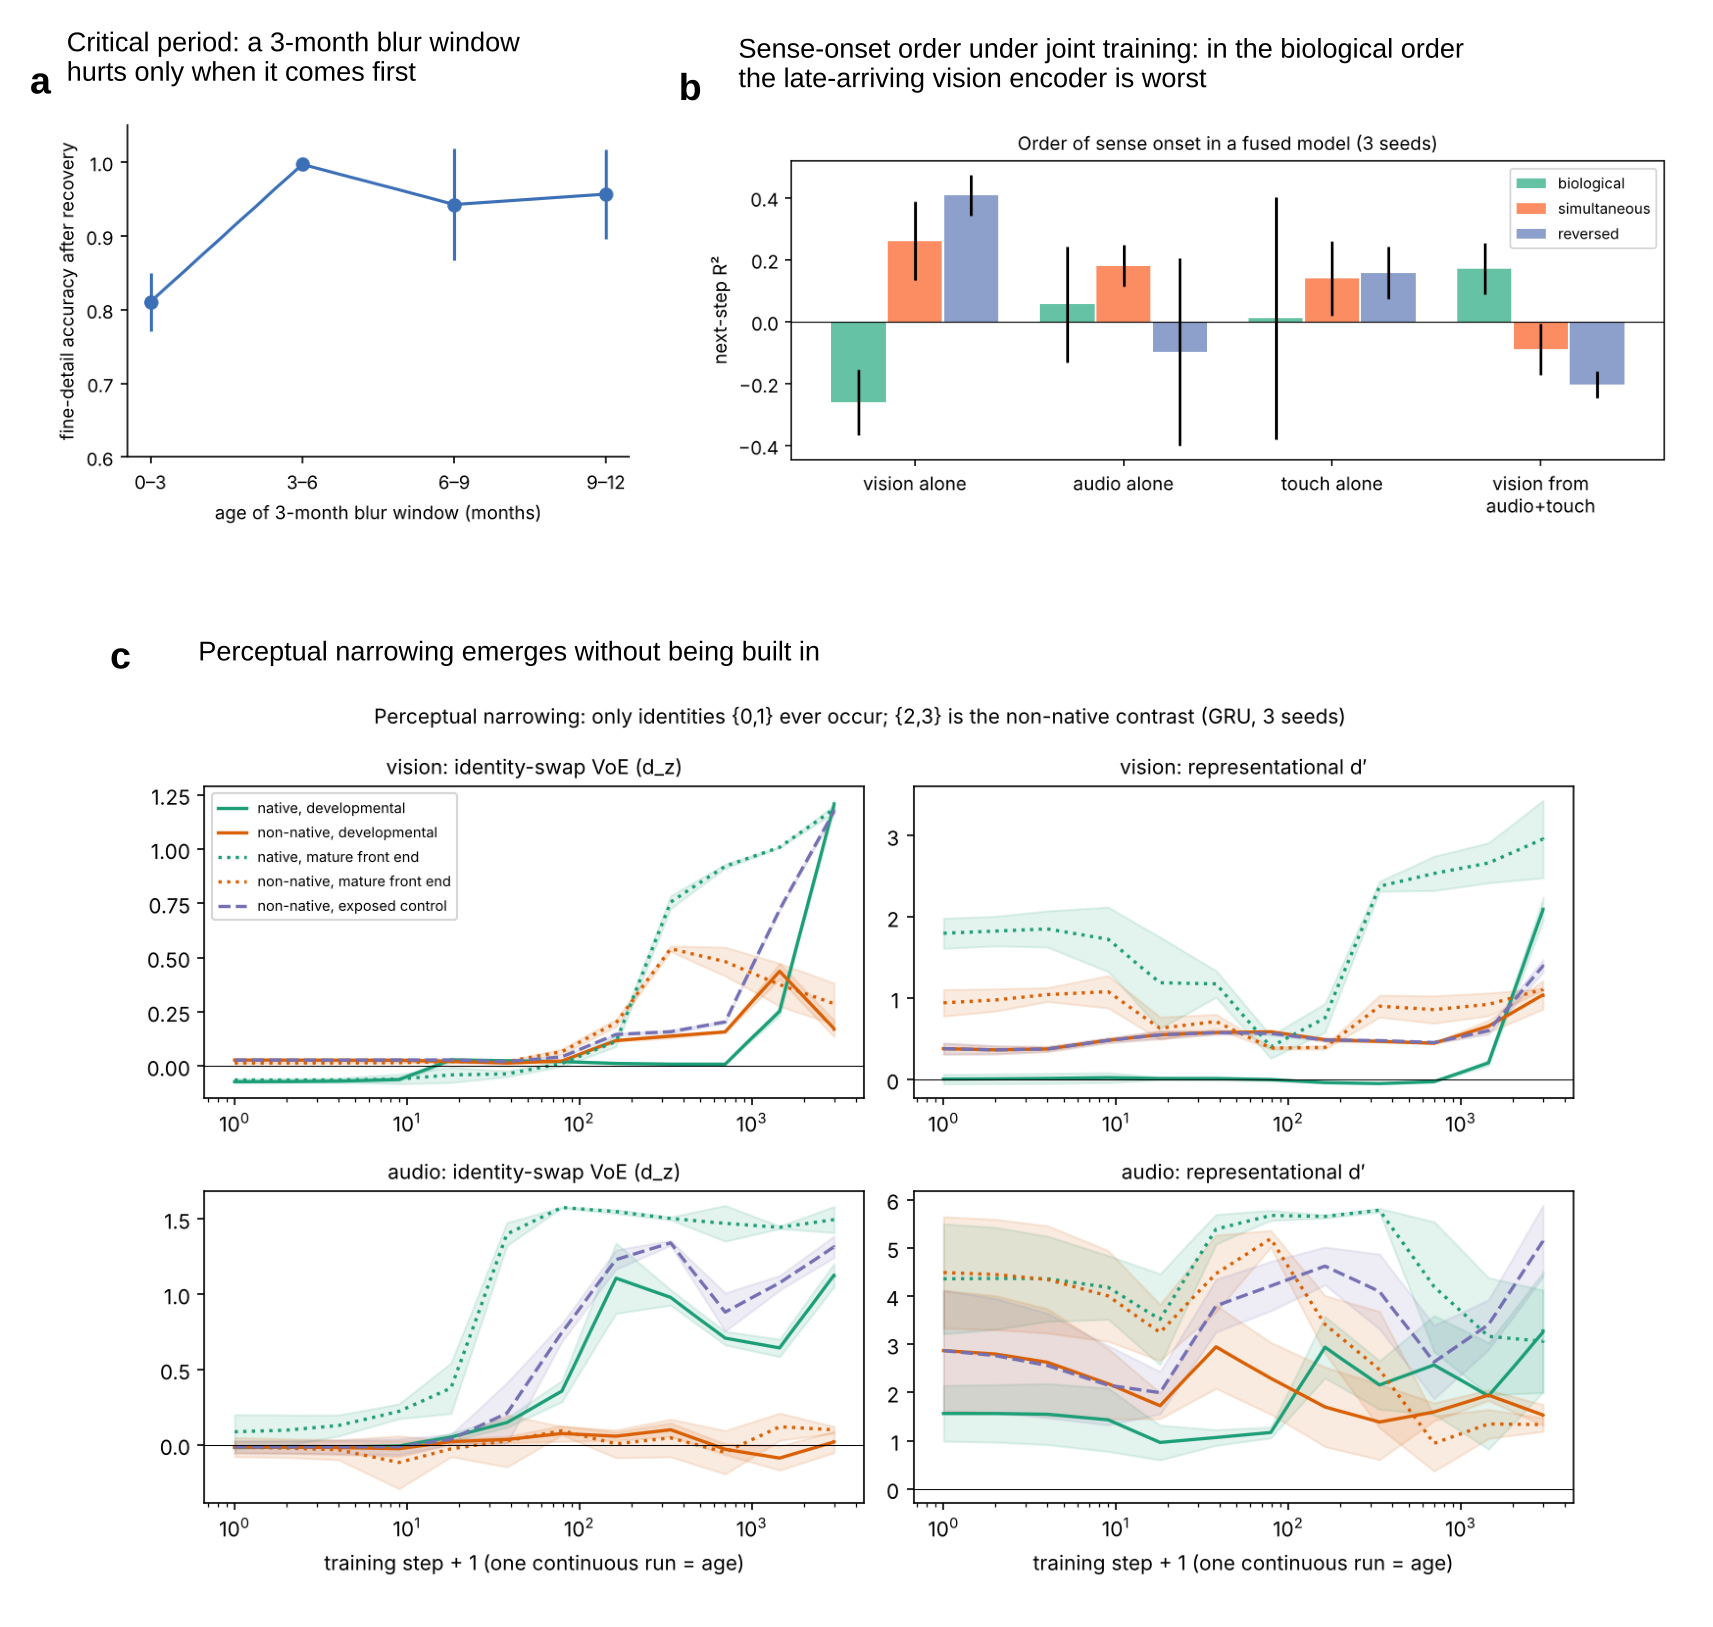
\includegraphics[width=\textwidth,height=0.78\textheight,keepaspectratio]{fig5_companion.png}
\caption{\textbf{Companion studies with independent code and stimuli.} \textbf{a}, Critical period: a 3-month window of blurred input, followed by 8 months of clear input, leaves a lasting deficit in fine-detail recognition only when the window comes first. \textbf{b}, Sense-onset order under joint training (next-step R\textsuperscript{2} of each encoder, and of vision predicted from hearing and touch): in the biological order, with vision arriving last, the vision encoder is worst; other orders favour the senses that arrive earlier. \textbf{c}, Perceptual narrowing: trained on two ``native'' identities only, surprise at a never-seen contrast first rises and then falls while the native contrast keeps improving.}
\end{figure}

Two companion studies with independent code and stimuli point the same way (Fig. 5). In compact networks on a shape-versus-texture task, the acuity schedule alone produced an infant-like curve whatever the capacity strategy, growing networks were slowest, and the same three months of blur caused a lasting deficit only when they came first: a critical period in a plain continuous run with no plasticity schedule, in line with critical periods reported in deep networks \autocite{achille2019critical}. In a two-sense version, the first sense crowded out the later one under joint training, and training each sense separately before fusing gave the best per-sense encoders, consistent with critical periods for multisensory integration \autocite{kleinman2023critical} and with accounts of limited early input \autocite{turkewitz1982limitations}. In a cross-sense study with violations applied to a latent world, memory was the only architectural requirement shared by all senses, and perceptual narrowing emerged without being built in.


\section{Discussion}

\textbf{So, do AI models learn like humans? Sometimes.} Table 3 lists the signatures we tested. Given infant-like input, small predictive world models reproduce the order of sensory maturation (by construction), a critical period, perceptual narrowing, the advantage of combining senses under occlusion, and a benefit of early degraded input in hearing. They do not reproduce expectations about hidden objects, and network growth, often proposed as the computational analogue of brain development, only slows them down.

\begin{longtable}[]{@{}
  >{\raggedright\arraybackslash}p{(\columnwidth - 4\tabcolsep) * \real{0.3333}}
  >{\raggedright\arraybackslash}p{(\columnwidth - 4\tabcolsep) * \real{0.3333}}
  >{\raggedright\arraybackslash}p{(\columnwidth - 4\tabcolsep) * \real{0.3333}}@{}}
\caption{Which infant signatures appear, and why.}\tabularnewline
\toprule\noalign{}
\begin{minipage}[b]{\linewidth}\raggedright
Infant signature
\end{minipage} & \begin{minipage}[b]{\linewidth}\raggedright
Present in our models?
\end{minipage} & \begin{minipage}[b]{\linewidth}\raggedright
What produces it
\end{minipage} \\
\midrule\noalign{}
\endfirsthead
\toprule\noalign{}
\begin{minipage}[b]{\linewidth}\raggedright
Infant signature
\end{minipage} & \begin{minipage}[b]{\linewidth}\raggedright
Present in our models?
\end{minipage} & \begin{minipage}[b]{\linewidth}\raggedright
What produces it
\end{minipage} \\
\midrule\noalign{}
\endhead
\bottomrule\noalign{}
\endlastfoot
Body senses first, vision last & Yes, by construction & Front-end tables \\
Slow early vision & Yes, beyond what the input requires & Input plus slow extraction by a predictive objective \\
Early immaturity helps later & In hearing (clean input), not in vision & Degraded input as augmentation \\
Critical period for early deprivation & Yes (companion study) & Continuous training; no plasticity schedule needed \\
Perceptual narrowing & Yes in vision, partly in hearing (companion study) & Training statistics \\
Multisensory advantage under occlusion & Yes & Fusion of frozen sense latents \\
Object permanence (surprise at vanishing) & No & Not produced by squared-error prediction \\
Growth as development & No: slower, half the compute & Zero-gradient start of new units \\
\end{longtable}

\textbf{What carries age.} Three independent synthetic settings agree that the infant-like shape of development comes from the input schedule, and that growing the network mostly slows learning. This fits neurobiology, in which neurons are not added after birth but the periphery, synapse density, myelination and plasticity change on per-sense clocks \autocite{huttenlocher1997regional,sydnor2021neurodevelopment,hensch2005critical}. Capacity should be a controlled factor, not the definition of age, and age is best represented as experience: checkpoints of one continuous run, not separate models per age, because only a continuous run can show history effects such as critical periods.

\textbf{What the constraints buy.} The costs and benefits are specific and modest. Immature early vision costs a little on clean input and buys no robustness we can establish; immature early hearing improves clean localisation. This is the honest form of ``starting small'' \autocite{elman1993learning,rohde1999language}: it is neither a free lunch nor a myth, and a full study must report both sides for every sense.

\textbf{Why expectations need more than prediction.} The failure of permanence is the most instructive result. The information is in the latent, yet the forecast does not use it, because a squared-error forecaster of pixels is rewarded for hedging. Objectives that predict in latent space \autocite{garrido2025intuitive}, represent uncertainty explicitly, or are trained on longer horizons should be tested against the same dissociating events.

\textbf{Limitations.} Everything is synthetic and small (at most 0.6 million parameters per sense) and evaluated mainly with linear probes, which measure decodability rather than behaviour. Hearing, touch and proprioception tables are placeholders, and ``months'' are training stages, not hours of experience. With 3 seeds per regime, several comparisons have large effect sizes but are not significant (Fig. 3c); we report them as estimates. An internal referee report and our responses are provided with the code (\texttt{report/PEER\_REVIEW.md}).

\textbf{Future work.} Extending the study will use experience-matched checkpoints of one continuous run per sense, sensory-immaturity and plasticity schedules as the main levers with capacity as an ablation, late fusion with sense-onset order as a factor, infant paradigms (violation of expectation, habituation, preferential looking) as the primary read-outs, and perceptual narrowing as the flagship cross-sense test. The data path runs from this synthetic nursery to an embodied infant simulator for touch and proprioception \autocite{mattern2024mimo} and to headcam corpora for vision and hearing \autocite{sullivan2021saycam,long2024babyview}.

\hypertarget{perspectives-from-mathematics-computer-science-and-neuroscience}{%
\subsection{Perspectives from mathematics, computer science and neuroscience}\label{perspectives-from-mathematics-computer-science-and-neuroscience}}

\textbf{Mathematics.}

\emph{Front ends bound what can be learned.} Let \(Y\) be a property of the scene (the toy's position) and \(\tilde O_a=\Phi_s(O;a)\) the filtered observation. For any learned representation \(Z=e(\tilde O_a)\), the data-processing inequality gives
\begin{equation}I(Z;Y)\le I(\tilde O_a;Y)\le I(O;Y).\end{equation}
The supervised ceiling in Fig. 2 estimates the middle term. The gap between ceiling and model is a property of learning; the ceiling itself is a property of the input.

\emph{Why a squared-error forecaster is not surprised.} The minimiser of \(\mathbb E\lVert \hat o_{t+1}-o_{t+1}\rVert^2\) over predictors of the past is the conditional mean \(\hat o_{t+1}^\star=\mathbb E[o_{t+1}\mid o_{\le t}]\). Behind a screen, let the toy reappear at frame \(t+1\) with probability \(p\). Then at each pixel the optimal forecast is a blend \(\hat o=(1-p)\,o^{\text{screen}}+p\,o^{\text{toy}}\), and the expected surprise is
\begin{equation}S_{\text{reappear}}=(1-p)^2\Delta^2,\qquad S_{\text{vanish}}=p^2\Delta^2,\qquad \Delta=o^{\text{toy}}-o^{\text{screen}},\end{equation}
so a model is more surprised by reappearance whenever \(p<\tfrac12\), which holds for most frames of an occlusion of uncertain length. A negative VoE index is the expected behaviour of a well-trained pixel forecaster, not a failure of training.

\emph{Function-preserving growth and its delay.} Widen a layer from \(n\) to \(n'\) units, \(W_1'=\begin{bmatrix}W_1\\R\end{bmatrix}\), \(W_2'=[\,W_2\;\;0\,]\). Then \(W_2'\phi(W_1'x)=W_2\phi(W_1x)\) for every \(x\). The gradient on the new incoming weights is
\begin{equation}\frac{\partial\mathcal L}{\partial R}=\big(\mathbf 0^\top\,\delta\big)\odot\phi'(Rx)\,x^\top=0,\end{equation}
so new units cannot learn until their outgoing weights move away from zero, which takes a number of updates that grows with the learning rate's inverse. The grown models pay this cost three times.

\textbf{Computer science.} Immature input is a curriculum in the sense of continuation methods: optimise a smoothed objective first, then track its minimiser as the smoothing is removed. Our hearing result (shuffled \ensuremath{\approx} ordered \textgreater{} adult) suggests that here the benefit is mostly augmentation. Growth trades accuracy for compute: at matched updates it costs about half the parameter-updates. Late fusion of separately trained senses avoids the competition between modalities seen under joint training, a known problem in multimodal learning, and modality dropout trains cross-modal fill-in.

\textbf{Neuroscience.} Each front end stands for a peripheral or early stage that matures on its own clock: the optics and cone mosaic of the eye and the immature visual cortex (acuity, contrast, colour) \autocite{banks1988optical}; the cochlea and binaural brainstem circuits (frequency resolution, high-frequency sensitivity, interaural differences); the shrinking receptive fields of the skin and somatosensory cortex; and muscle-spindle and joint signals for proprioception. The memory window stands for working memory and persistent activity; the fusion model for multisensory integration in the superior colliculus and superior temporal sulcus. The brain grows synapses and then prunes them \autocite{huttenlocher1997regional} rather than adding neurons, and closes plasticity on per-sense schedules governed by excitatory-inhibitory balance \autocite{hensch2005critical}. Our growth ablation is therefore a test of an engineering idea, not of biology; the biologically motivated levers are sensory immaturity and plasticity schedules. Predictive coding frames all of this: each world model minimises the error of its own predictions, and violation-of-expectation is the behavioural read-out of that error.


\textbf{General.} During the preparation of this work, the author used an AI assistant (Claude, Anthropic) to help write and run analysis code, draw figures and draft text. The author reviewed and edited the content and takes full responsibility for the content of the publication.

\textbf{Author contributions.} S. Mohapatra conceived the study, directed the work and approved the final text.

\textbf{Funding.} This work received no specific funding and was carried out independently.

\textbf{Competing interests.} The author declares that there is no conflict of interest regarding the publication of this article.

\textbf{Data availability.} All code, configurations, aggregated results and trained checkpoints are available at github.com/pikulsomesh/developmental-world-models. The data are synthetic and are regenerated by the code from the random seeds listed in the repository.

Extended Data Figs. 1 to 3 (below), \texttt{report/REFERENCES\_VERIFIED.md} (the reference-verification log) and \texttt{report/PEER\_REVIEW.md} (an internal referee report with responses) are available in the repository.

\clearpage
\section*{Extended Data (Supplementary Figures)}
\setcounter{figure}{0}
\renewcommand{\thefigure}{S\arabic{figure}}

\begin{figure}[tbp]
\centering
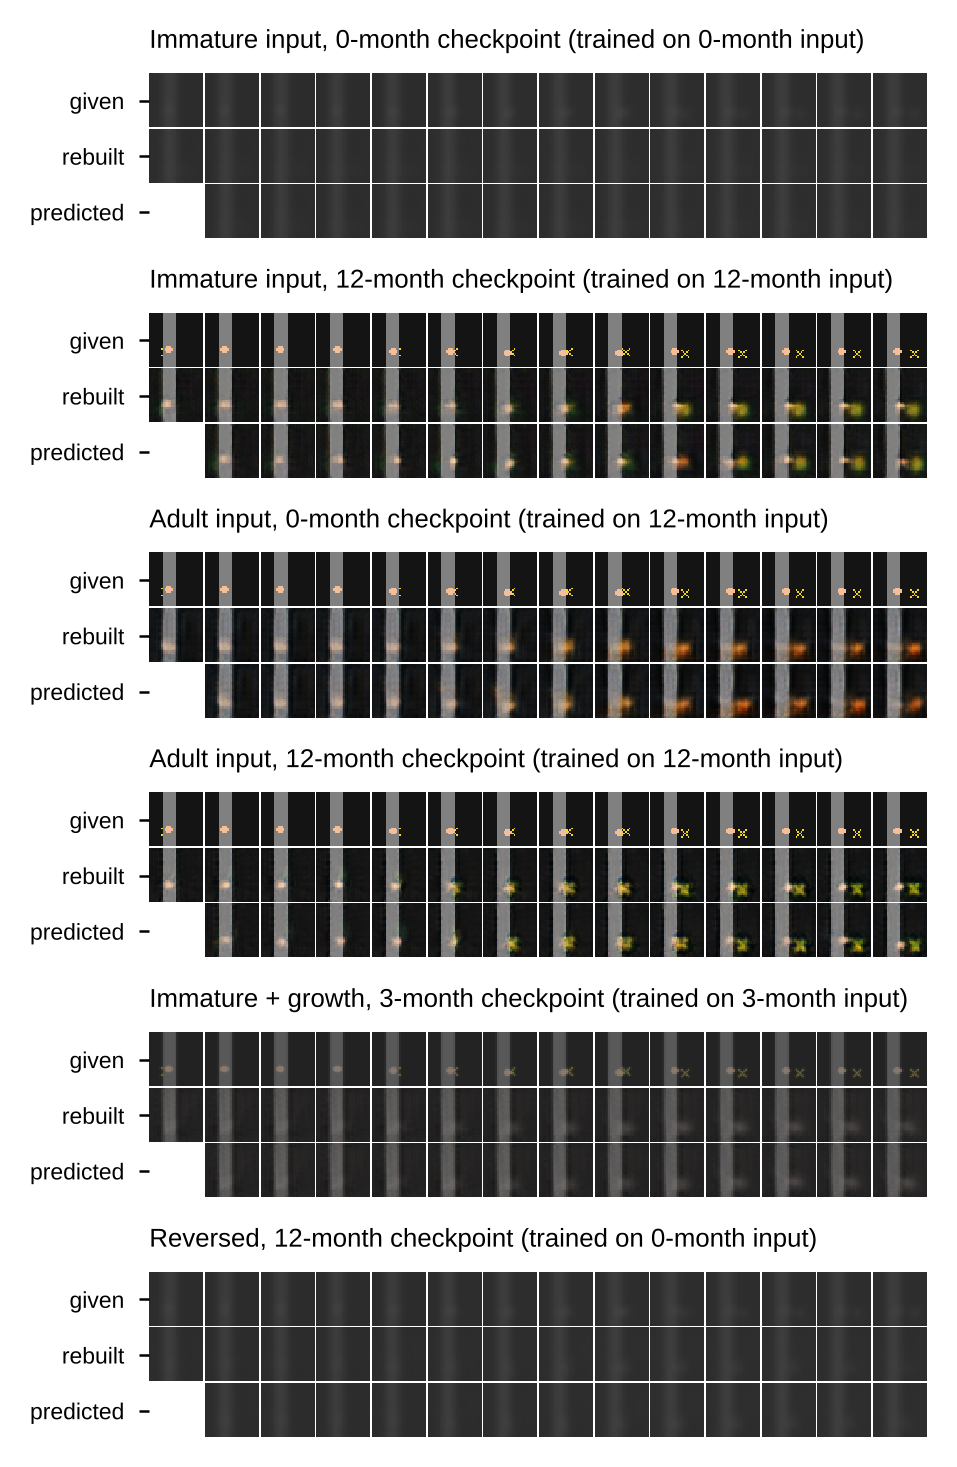
\includegraphics[width=\textwidth,height=0.78\textheight,keepaspectratio]{ed1_model_outputs.png}
\caption{\textbf{What the vision models see, rebuild and predict.} For selected regimes and checkpoints: the input given (at the age that stage was trained on), the reconstruction from the latent, and the one-step prediction, for the first 14 frames of one episode.}
\end{figure}

\begin{figure}[tbp]
\centering
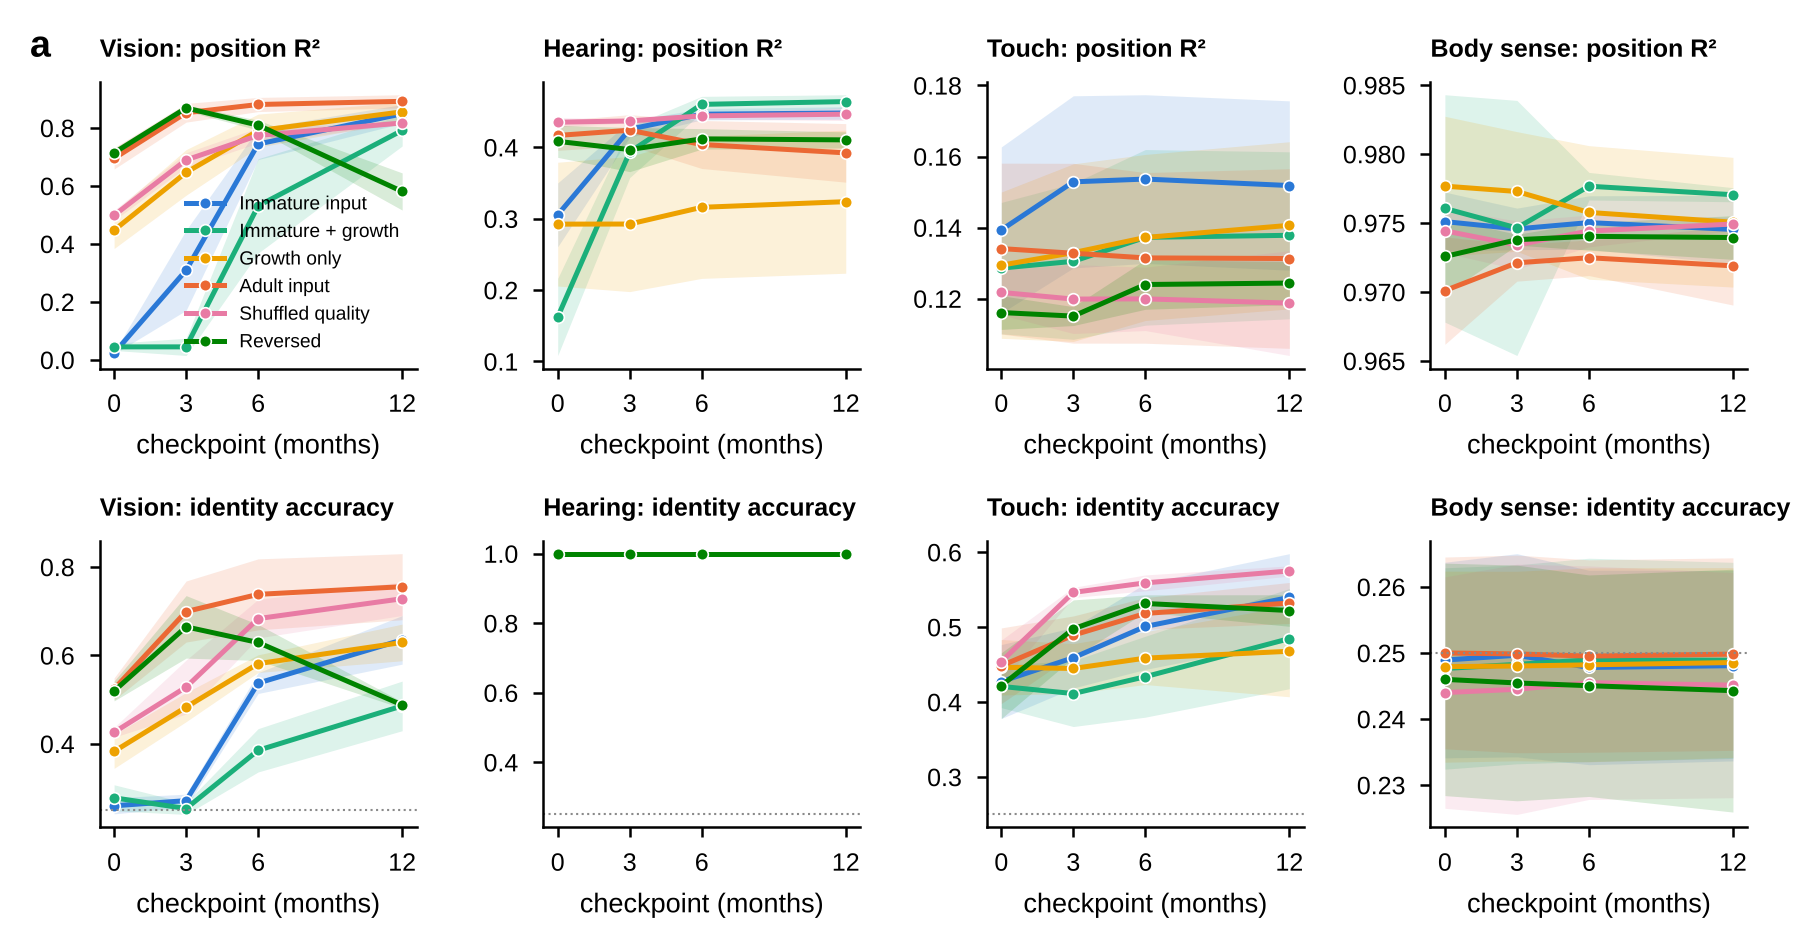
\includegraphics[width=\textwidth,height=0.78\textheight,keepaspectratio]{ed2_all_senses.png}
\caption{\textbf{All senses, all regimes.} Position R\textsuperscript{2} (top) and identity accuracy (bottom; dotted, chance) per checkpoint.}
\end{figure}

\begin{figure}[tbp]
\centering
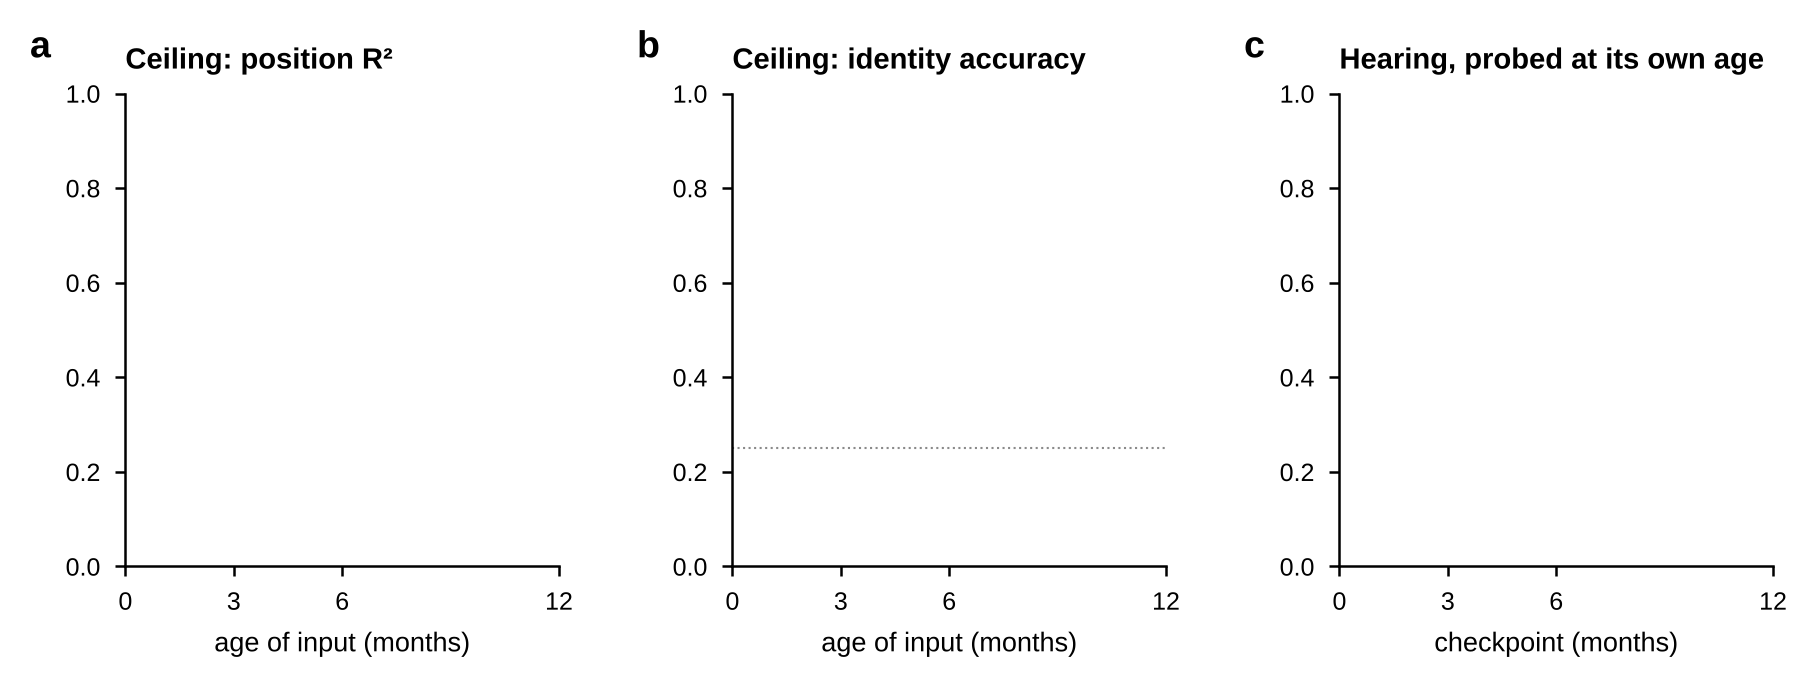
\includegraphics[width=\textwidth,height=0.78\textheight,keepaspectratio]{ed3_ceiling_ownage.png}
\caption{\textbf{Information ceilings and own-age probes.} \textbf{a}, \textbf{b}, Supervised ceilings per sense and age. \textbf{c}, Hearing probed on own-age input.}
\end{figure}


\printbibliography

\end{document}
